%	PACKAGES AND OTHER DOCUMENT CONFIGURATIONS

\documentclass[11pt, a4paper,twocolumn]{article} % 10pt font size (11 and 12 also possible), A4 paper (letterpaper for US letter) and two column layout (remove for one column) Use additional titlepage argument to generate this
%\documentclass[12pt, a4paper,twocolumn,titlepage]{article}

%%%%%%%%%%%%%%%%%%%%%%%%%%%%%%%%%%%%%%%%%
% Wenneker Article
% Structure Specification File
% Version 1.0 (28/2/17)
%
% This file originates from:
% http://www.LaTeXTemplates.com
%
% Authors:
% Frits Wenneker
% Vel (vel@LaTeXTemplates.com)
%
% License:
% CC BY-NC-SA 3.0 (http://creativecommons.org/licenses/by-nc-sa/3.0/)
%
%%%%%%%%%%%%%%%%%%%%%%%%%%%%%%%%%%%%%%%%%

%----------------------------------------------------------------------------------------
%	PACKAGES AND OTHER DOCUMENT CONFIGURATIONS
%----------------------------------------------------------------------------------------

\usepackage[english]{babel} % English language hyphenation

\usepackage{microtype} % Better typography

\usepackage{verbatim} % Allows mulitline commenting

\usepackage{amsmath,amsfonts,amsthm} % Math packages for equations

\usepackage[svgnames]{xcolor} % Enabling colors by their 'svgnames'

\usepackage[hang, small, labelfont=bf, up, textfont=it]{caption} % Custom captions under/above tables and figures

\usepackage{subcaption}

\usepackage{booktabs} % Horizontal rules in tables

\usepackage{lastpage} % Used to determine the number of pages in the document (for "Page X of Total")

\usepackage{graphicx} % Required for adding images

\usepackage{enumitem} % Required for customising lists
\setlist{noitemsep} % Remove spacing between bullet/numbered list elements

\usepackage{sectsty} % Enables custom section titles
\allsectionsfont{\usefont{OT1}{phv}{b}{n}} % Change the font of all section commands (Helvetica)

\usepackage{bm} % Used for bold font in math environments

\usepackage{siunitx} % Used for SI units

\usepackage{tikz} % Used for tikz diagrams
\usetikzlibrary{calc} % Enable math in tikz code

\newcommand*{\subscript}[1]{\ensuremath{_\textrm{{\scriptsize #1}}}}  %Non italic subscripts

%----------------------------------------------------------------------------------------
%	MARGINS AND SPACING
%----------------------------------------------------------------------------------------

\usepackage{geometry} % Required for adjusting page dimensions

\geometry{
	top=1cm, % Top margin
	bottom=1.5cm, % Bottom margin
	left=2cm, % Left margin
	right=2cm, % Right margin
	includehead, % Include space for a header
	includefoot, % Include space for a footer
	%showframe, % Uncomment to show how the type block is set on the page
}

\setlength{\columnsep}{7mm} % Column separation width

%----------------------------------------------------------------------------------------
%	FONTS
%----------------------------------------------------------------------------------------

\usepackage[T1]{fontenc} % Output font encoding for international characters
\usepackage[utf8]{inputenc} % Required for inputting international characters

\usepackage{XCharter} % Use the XCharter font

%----------------------------------------------------------------------------------------
%	HEADERS AND FOOTERS
%----------------------------------------------------------------------------------------

\usepackage{fancyhdr} % Needed to define custom headers/footers
\pagestyle{fancy} % Enables the custom headers/footers

\renewcommand{\headrulewidth}{0.0pt} % No header rule
\renewcommand{\footrulewidth}{0.4pt} % Thin footer rule

\renewcommand{\sectionmark}[1]{\markboth{#1}{}} % Removes the section number from the header when \leftmark is used

%\nouppercase\leftmark % Add this to one of the lines below if you want a section title in the header/footer

% Headers
\lhead{} % Left header
\chead{\textit{\thetitle}} % Center header - currently printing the article title
\rhead{} % Right header

% Footers
\lfoot{} % Left footer
\cfoot{} % Center footer
\rfoot{\footnotesize Page \thepage\ of \pageref{LastPage}} % Right footer, "Page 1 of 2"

\fancypagestyle{firstpage}{ % Page style for the first page with the title
	\fancyhf{}
	\renewcommand{\footrulewidth}{0pt} % Suppress footer rule
}

%----------------------------------------------------------------------------------------
%	TITLE SECTION
%----------------------------------------------------------------------------------------

\newcommand{\authorstyle}[1]{{\large\usefont{OT1}{phv}{b}{n}\color{NavyBlue}#1}} % Authors style (Helvetica)

\newcommand{\institution}[1]{{\footnotesize\usefont{OT1}{phv}{m}{sl}\color{Black}#1}} % Institutions style (Helvetica)

\usepackage{titling} % Allows custom title configuration

\newcommand{\HorRule}{\color{SteelBlue}\rule{\linewidth}{1pt}} % Defines the gold horizontal rule around the title

\pretitle{
	\vspace{-30pt} % Move the entire title section up
	\HorRule\vspace{10pt} % Horizontal rule before the title
	\fontsize{32}{36}\usefont{OT1}{phv}{b}{n}\selectfont % Helvetica
	\color{Navy} % Text colour for the title and author(s)
}

\posttitle{\par\vskip 15pt} % Whitespace under the title

\preauthor{} % Anything that will appear before \author is printed

\postauthor{ % Anything that will appear after \author is printed
	\vspace{10pt} % Space before the rule
	\par\HorRule % Horizontal rule after the title
	\vspace{20pt} % Space after the title section
}

%----------------------------------------------------------------------------------------
%	ABSTRACT
%----------------------------------------------------------------------------------------

\usepackage{lettrine} % Package to accentuate the first letter of the text (lettrine)
\usepackage{fix-cm}	% Fixes the height of the lettrine

\newcommand{\initial}[1]{ % Defines the command and style for the lettrine
	\lettrine[lines=3,findent=4pt,nindent=0pt]{% Lettrine takes up 3 lines, the text to the right of it is indented 4pt and further indenting of lines 2+ is stopped
		\color{NavyBlue}% Lettrine colour gold DarkGoldenRod
		{#1}% The letter
	}{}%
}

\usepackage{xstring} % Required for string manipulation

\newcommand{\lettrineabstract}[1]{
	\StrLeft{#1}{1}[\firstletter] % Capture the first letter of the abstract for the lettrine
	\initial{\firstletter}\textbf{\StrGobbleLeft{#1}{1}} % Print the abstract with the first letter as a lettrine and the rest in bold
}

%	BIBLIOGRAPHY

\usepackage[backend=biber,style=phys,natbib=true,doi=false]{biblatex} 
%Can equally use numeric citation style without extra phys packaging (but doesn't change capitalisation), or authoryear for alphabetical listing without the codes (resembles APA)

%\addbibresource{references.bib} % The filename of the bibliography

\usepackage[autostyle=true]{csquotes} % Required to generate language-dependent quotes in the bibliography


%   CODE LISTING
\usepackage[title]{appendix} %in appendix

\usepackage{listings}
\usepackage{pythontex}

\usepackage{setspace}
\definecolor{Code}{rgb}{0,0,0}
\definecolor{Decorators}{rgb}{0.5,0.5,0.5}
\definecolor{Numbers}{rgb}{0.5,0,0}
\definecolor{MatchingBrackets}{rgb}{0.25,0.5,0.5}
\definecolor{Keywords}{rgb}{0,0,1}
\definecolor{self}{rgb}{0,0,0}
\definecolor{Strings}{rgb}{0.874, 0.533, 0.047}
\definecolor{Comments}{rgb}{0,0.63,0} %was 1 at the end
\definecolor{Definitions}{rgb}{1,0,0}
\definecolor{Backquotes}{rgb}{0,0,0}
\definecolor{Classname}{rgb}{0.454, 0.090, 0.592}  % odd
\definecolor{FunctionName}{rgb}{0.454, 0.090, 0.592} % odd
\definecolor{Operators}{rgb}{0.090, 0.592, 0.560} % odd
\definecolor{Background}{rgb}{0.98,0.98,0.98}
%\lstdefinelanguage{Python}{  %replaces two lines below
\lstset{
	language=Python,
	showspaces=false,
	showtabs=false,
	showstringspaces=false,
	%frame=l,   % gives black line by text
	tabsize=4,
	% Basic
	basicstyle=\ttfamily\small\setstretch{1},  % determines font and other style
	%backgroundcolor=\color{Background},      % gives background colour for all code
	% Comments
	commentstyle=\color{Comments}\slshape,
	% Strings
	stringstyle=\color{Strings},
	morecomment=[s][\color{Numbers}]{"""}{"""},
	morecomment=[s][\color{Numbers}]{'''}{'''},
	% keywords
	morekeywords={import,from,class,def,for,while,if,is,in,elif,else,not,and,or,print,break,continue,return,True,False,None,access,as,del,except,exec,finally,global,import,lambda,pass,print,raise,try,assert},
	keywordstyle={\color{Keywords}\bfseries},
	% additional keywords
	morekeywords={[2]@invariant,pylab,numpy,np,scipy},
	keywordstyle={[2]\color{Decorators}\slshape},
	emph={self},
	emphstyle={\color{self}\slshape},
	%
}
 % Specifies the document structure and loads requires packages
\graphicspath{{"/Users/Kit/OneDrive/Documents/Computing/Trojan Asteroids/Report/Figures"}}
\newcommand*{\subscript}[1]{\ensuremath{_\textrm{{\scriptsize #1}}}}

\usepackage{bm}
\usepackage{tikz}
\usetikzlibrary{calc}

%	ARTICLE INFORMATION

\title{Modelling the Trojan Asteroids}
%\subtitle{Blue Organic Light Emitting Diodes using Thermally Activated Delayed Fluorescence}

%\author{
	%\authorstyle{Christopher Gallagher}}
\author{\authorstyle{Christopher Gallagher} 
	\institution{University of Cambridge}}
% Example of a one line author/institution relationship
%\author{\newauthor{John Marston} \newinstitution{Universidad Nacional Autónoma de México, Mexico City, Mexico}}

\date{\today} % Add a date here if you would like one to appear underneath the title block, use \today for the current date, leave empty for no date
\usepackage[english]{babel}
\usepackage{tabularx}
%\usepackage[backend=biber,doi=false]{biblatex}
\addbibresource{references.bib}
%\AtBeginBibliography{\small}
%----------------------------------------------------------------------------------------
\begin{document}

\maketitle % Print the title

\thispagestyle{firstpage} % Apply the page style for the first page (no headers and footers)

%	ABSTRACT

\lettrineabstract{Trojan asteroids are v important. I'm going to make that paragraph a little longer to fill out the space in case this is forming some kind of error. i really hope this is long enough.}

%	ARTICLE CONTENTS

%Use https://leancrew.com/all-this/2016/08/lagrange-points-redux/ to create your own contour plot?
\section{Introduction}
The Jupiter trojans, commonly known as the Trojan asteroids, are two large groups of asteroids that share the planet Jupiter's orbit around the Sun in a 1:1 orbit resonance. These two groups are called the Greeks and the Trojans, named after opposing sides in the mythological Trojan war, and lead/trail Jupiter respectively in its orbit. They correspond to Jupiter's two stable Lagrange points: L\subscript{4}, lying 60° ahead of the planet in its orbit, and L\subscript{5}, 60° behind, with asteroids distributed in two elongated, curved regions around these Lagrangian points. 

The first Jupiter trojan, 588 Achilles, was discovered in 1906 by the German astronomer Max Wolf \cite{Nicholson1961}, and a total of 7642 Jupiter trojans have been found as of February 2020 \cite{IAU2020}.

Research into Jupiter's trojan asteroids continues, with the particular focus on their origins reliant on an understanding of their orbit stability \cite{DiSisto2019}, \cite{Nesvorn2018}. This informs studies into their composition \cite{Brown2016}, as travel to these asteroids is considered for their potential in mineral mining \cite{Okada2017} \cite{Levison2016}. 

The purpose of this report is to use numerical simulation techniques to investigate the stability of orbits about these Lagrange points, demonstrating the asteroid oscillate about these points under small perturbations and quantifying the absolute distance of the asteroids from the Lagrange point (the wander) during their orbits. The impact of variation in planetary/solar mass on asteroid orbit stability will also be considered. \textit{Signpost what is included in each section?}

% \cite{Nakamura2008} gives spatial distribution

\section{Theoretical Background?}

\subsection{Lagrange Points}
The asteroids exist at/near Lagrange points, defined in Lagrange's initial analysis of the three-body problem in 1772 \cite{Lagrange1772}, were he demonstrated the existence of five equilibrium points for an object of negligible mass orbiting under the gravitational effect of two larger masses. Three of these equilibrium points, L\subscript{1}-L\subscript{3} lie on the line joining the two masses, while each of the remaining two points, L\subscript{4} and L\subscript{5}, lie at the apex of an equilateral triangle with base equal to the separation of the two masses (see Figure \ref{fig:lagrangepoints}). Despite all these points being potential maxima, stable motion is possible around L\subscript{4} and L\subscript{5} due to the Coriolis force \cite{Lissauer2014}.
%lissauer also says stability is provided that the most massive body has at least 25 times the mass of the secondary

\begin{figure}[h]
	\centering
	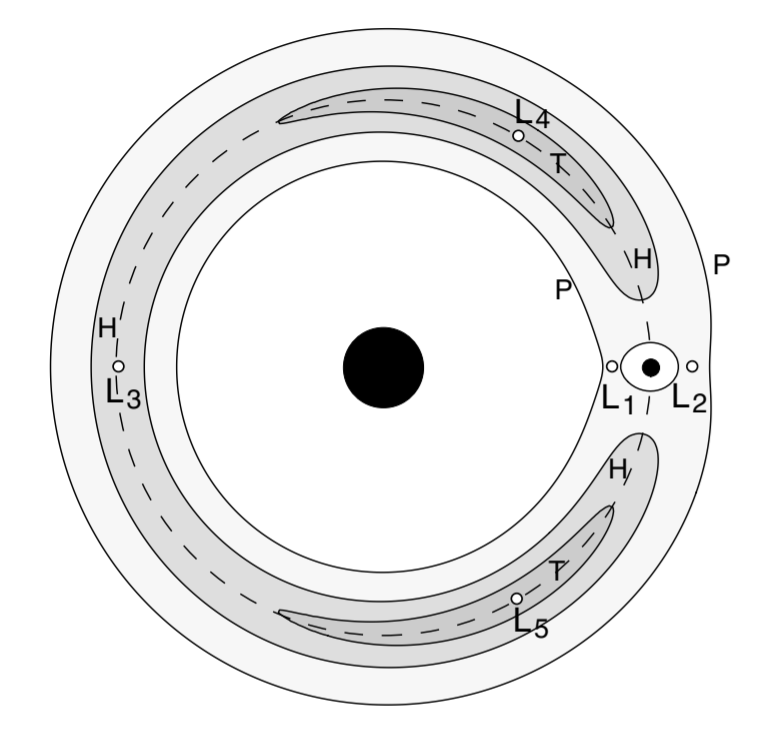
\includegraphics[width=\linewidth]{Figures/lagrange_points}
	\caption{The location of the five Lagrange equilibrium points in the circular-restricted three-body problem. The solar and planetary masses are denoted by the large and small filled circles, and the letters P, H, and T denote passing, horseshoe, and tadpole orbits respectively. Note that the two masses form an equilateral triangle with each of the L\subscript{4} and L\subscript{5} points. Reproduced from Marzari et al. \cite{Marzari2002}}
	\label{fig:lagrangepoints}
\end{figure}

While orbits between Lagrange points are also possible, this report will focus on the tadpole orbits observed as asteroids deviate from L4 and L5 \cite{Murray1999}. \textit{More detail?}


\subsection{Theoretical Model}
The three body problem, where the dynamics of three interacting bodies are determined given their initial positions and velocities, has no analytical (closed-form) solution in the general case \cite{Barrow2008}.

In this report, I will consider the circular, restricted, three-body problem, where two of the bodies move in circular, coplanar orbits about their common centre of mass, unaffected by the negligible mass of the third body. I will also assume that all interactions are via Newtonian gravity.

Rescaled solar system units are used for mathematical ease, so distances are measured in astronomical units (AU), time in earth years and mass in multiples of the solar mass.

The system of differential coordinates determine the position and velocity of the asteroids, with two equations per spatial coordinate.
\begin{equation}
\frac{dr_{i}}{dt} = v_{i}, \frac{dv_{i}}{dt} = g_{i}, \quad i = x,y 
\end{equation}

In this, $g_{i}$ is given by:
\begin{equation}
\textbf{g}= - \frac{G M_{s}}{\lvert \textbf{r} - \textbf{r}_{s} \rvert ^{3}} (\textbf{r} - \textbf{r}_{s})
		 - \frac{G M_{p}}{\lvert \textbf{r} - \textbf{r}_{p} \rvert ^{3}} (\textbf{r} - \textbf{r}_{p})
\end{equation}
where the subscripts \textit{s} and \textit{p} refer to solar and planetary properties respectively.

We may also consider a frame rotating at the same speed as the massive bodies. As there is 1:1 orbital resonance between Jupiter and the asteroids, all three bodies are stationary in this frame. This significantly increases the accuracy of numerical simulations, as \textbf{WHY}

When transforming into this rotating non-inertial frame, $g_{i}$ gains an additional virtual force term with coupling between the spatial coordinates. This is given below as the sum of the centripetal and Coriolis forces:

\begin{equation}
\Delta g_{i} = \Omega^{2} r_{i} - 2[\bm{\Omega} \times \textbf{v}]_{i}
\end{equation}
where $\Omega$ is the angular speed of the rotating frame, and $\textbf{v}$ is the velocity of the asteroid within this frame. 


\subsubsection{Assumptions - FIX}
\begin{itemize}
	\item Circular orbit
	\item Constant Jupiter-Sun separation
	\item Coplanar orbits
	\item Negligible asteroid mass
	\item Newtonian gravity
\end{itemize}

I also applied the following symmetries:
trojan and greek symmetry (analysis focused on greeks)
rotational symmetry - arbitrary initial point 
direction of orbit
"The combination of these symmetries allows the problem to be simplified. Such that
only the Greeks, orbiting counter-clockwise, with perturbations at t = 0, need to be
investigated.
"

\subsection{Orbit Geometry}
As the three bodies considered here form an equilateral triangle in the initial equilibrium state, as depicted in Figure \ref{fig:geometry}, we can derive the polar coordinates of each body with respect to the centre of mass about which the bodies orbit.

\begin{figure}
	\centering
	\resizebox{\columnwidth}{!}{%
		\begin{tikzpicture}
		\draw (0,0) -- (6,0) -- (3, {6*sin(60)} ) node[above]{Asteroids} node[midway,right]{$a$} -- cycle node[midway,left]{$a$};
		\draw  (1,0) arc (0:60:1cm)  ;
		%\node [label={[shift = {(10mm,5mm)}]{$\frac{\pi}{3}$}}] {};
		\node [label={[shift = {(13:11mm)}]{$\frac{\pi}{3}$}}] {};
		\node [label={[shift = {(-7mm,-7mm)}]{Sun}}] {};
		\node [label={[shift = {(67mm,-7mm)}]{Planet}}] {};
		
		\fill[gray] ({6*(1/4)}, 0) circle (0.5mm);
		\draw[gray] ({6*(1/4)}, 0) -- (3, {6*sin(60)} ) node[midway,left]{$r_{a}$};
		\draw[dashed, gray] (3, 0) -- (3, {6*sin(60)} )node[midway,right]{$\frac{\sqrt{3}a}{2}$};
		\draw[gray]  ({6*(1/4) + 1}, 0) arc (0:{atan(4*sin(60))}:1cm)  ;
		\node [label={[gray, shift = {(25mm,3mm)}]$\theta$}] {};
		\draw[gray] (2.75,0) -- (2.75, 0.25) -- (3, 0.25);
		
		\draw[arrows=<-](0,-0.5)--(0.53,-0.5);
		\node at (0.75, -0.5) {$R_s$};
		\draw[arrows=->](1.0,-0.5)--(1.48,-0.5);
		
		\draw[arrows=<-](1.52,-0.5)--(3.53,-0.5);
		\node at (3.75, -0.5) {$R_p$};
		\draw[arrows=->](4.00,-0.5)--(6,-0.5);
		
		%\draw[arrows=<-](0,-1)--(2.88,-1);
		%\node at (3, -1) {$a$};
		%\draw[arrows=->](3.1,-1)--(6, -1);
		
		\fill[black] (0,0) circle (3.5mm);% node[anchor=north west] {Sun};
		\fill[black] (6,0) circle (1mm);
		\fill[black] (3, {6*sin(60)} ) circle (0.5mm);
		
		\end{tikzpicture}
	}	
	\caption{A geometric depiction of the three-body system, in the case where the planet has a mass equal to a third of the sun, and asteroids are considered at the L\subscript{4} point. $ R_{s} $ and $ R_{p}$ denote the (fixed) radii from the centre of mass (the grey point) to the Sun and the planet respectively, while $ r_{a} $ denotes the radius of the asteroids.}
	\label{fig:geometry}
\end{figure}

Using standard trigonometric relations, it is simple to show that the values $ r_{a} $ and $ \theta $ are given by:

\begin{equation}
r_{a} = \sqrt{a^{2} + R_{s} R_{p}} , \enspace \theta =  \tan^{-1} \left( \frac{a \sin(\frac{\pi}{3})}{R_{p} - \frac{a}{2}} \right)
\end{equation}

Furthermore, the Lagrange point in Cartesian coordinates based about the centre of mass is easily found to be:

\begin{equation}
(x,y) = \left( R_{p} - \frac{a}{2}, \frac{ \sqrt{3} a}{2} \right)
\end{equation}

Finally, equating the gravitational and centripetal forces on the planet allows the derivation of its (and all other bodies') orbital velocity:

\begin{equation}
\Omega = \sqrt{\frac{G (M_{s} + M_{p})}{a^{3}}}
\end{equation}

\section{Methodology}
\subsection{Integration Method}
%Put this with theory as "numerical methods"?
%Then all theory could be in methodology?
The default solver is RK45 (an explicit Runge-Kutta method of order 5(4) \cite{Dormand1980}) however this is non-stiff, giving a deviation in asteroid position (from the Lagrange point) in the order of $ 10^{-4}$ AU in the rotating frame over 50 years. This is larger than expected, suggesting the system of equations requires an unreasonable small step size for  numerically stability with respect to this numerical method, even regions where the solution curve is smooth \cite{Lambert1991}. This suggests the system is stiff, and solvers designed for this typically do more work per step, allowing them to take much larger steps, and have improved numerical stability compared to the non-stiff solvers \cite{Byrne1987}. 

Instead the stiff "Radau" solver (an implicit Runge-Kutta method of the Radau IIA family of order 5 \cite{Hairer2010}) is used for increased stability \cite{Frank1985}, and achieves a deviation in asteroid position in the order of $ 10^{-13}$ AU instead. This also ensures stability in the rotating frame, with deviations of 0.76\% in asteroid separation from Jupiter over $ 10^{3} $ years, compared to 53\% for the best non-stiff solvers.

%Can add more detail on A vs B stability (I believe B stability is relevant here but maybe check this)
\section{Results}
\subsection{Orbit Stability}
\subsection{Wander Analysis}
\subsubsection{Perturbations in z-direction}

\section{Discussion}
\section{Conclusion}



%Talk about animations here too? or after solver method
\printbibliography

\end{document}

%%%%%%%%%%%%%%%%%%%%%%%%%%%%%%%%%%%%%%%%%
% Wenneker Article
% LaTeX Template
% Version 2.0 (28/2/17)
%
% This template was downloaded from:
% http://www.LaTeXTemplates.com
%
% Authors:
% Vel (vel@LaTeXTemplates.com)
% Frits Wenneker
%
% License:
% CC BY-NC-SA 3.0 (http://creativecommons.org/licenses/by-nc-sa/3.0/)
%
%%%%%%%%%%%%%%%%%%%%%%%%%%%%%%%%%%%%%%%%%
